\documentclass[a4paper,10pt]{article}

\usepackage[T1]{fontenc}
\usepackage[utf8]{inputenc}
\usepackage[english]{babel}

\usepackage{geometry}
\geometry{
    textwidth=190mm,
    textheight=267mm,
	inner=10mm,
	outer=10mm,
	top=10mm,
	bottom=20mm
}
\usepackage{fancyhdr}
\usepackage{graphicx}
\usepackage{fontawesome}
\usepackage{hyperref}
\hypersetup{
	colorlinks = true,
	urlcolor = cyan,
	linkcolor = black,
}

%%%%%%%%%%%%%%%%%%%% - Usage Changes - %%%%%%%%%%%%%%%%%%%%
\newcommand{\professional}{Mateus Souza Oliveira}
\newcommand{\age}{25}
\newcommand{\address}{Rodovia Amaro Antônio Vieira, 2593 -- Itacorubi. Florianópolis, Santa Catarina, Brazil}
\newcommand{\phone}{+55 (48) 9 9810-2694}
\newcommand{\email}{matews1943@gmail.com}
\renewcommand{\date}{\today}
\newcommand{\about}{
    Proactive, detailed, determined and always seeking to improve myself. Currently, I am working as a junior software developer at CERTI Foundation. \\

    I am interested in learning Dart (Flutter) and C. I prefer to work on Linux. Check some of my projects in my GitHub repository and in my personal website!
	\vspace{2\baselineskip}
}
%%%%%%%%%%%%%%%%% - End of Usage Changes - %%%%%%%%%%%%%%%%

\setlength{\fboxrule}{2pt}
\setlength{\fboxsep}{0pt}

\fancyhead{} % Header: reset
\fancyfoot{} % Footer: reset
\fancyfoot[C]{Page \thepage \ of \pageref{lastPage}} % Footer: center
\fancyfoot[R]{Made with \LaTeX} % Footer: right
\fancyfoot[L]{Updated in \date} % Footer: left
\renewcommand{\headrulewidth}{0pt} % Header line thickness
\renewcommand{\footrulewidth}{0.4pt} % Footer line thickness
\pagestyle{fancy} % Sets the page style

\newcommand{\createSection}[4][0]{
    \noindent
	\begin{minipage}{0.16\linewidth}
		\large{\textbf{#2}}
		\vspace{#3\baselineskip}
	\end{minipage}
	\hfill
	\begin{minipage}{0.79\linewidth}
		#4
		\ifnum0#1>0 { \hrule {\ } } \fi
	\end{minipage}
	\vspace{\baselineskip}
}

\begin{document}

	\noindent
	\fbox{
	\hspace*{-3.35\fboxrule}
	\begin{minipage}{0.3\linewidth}
		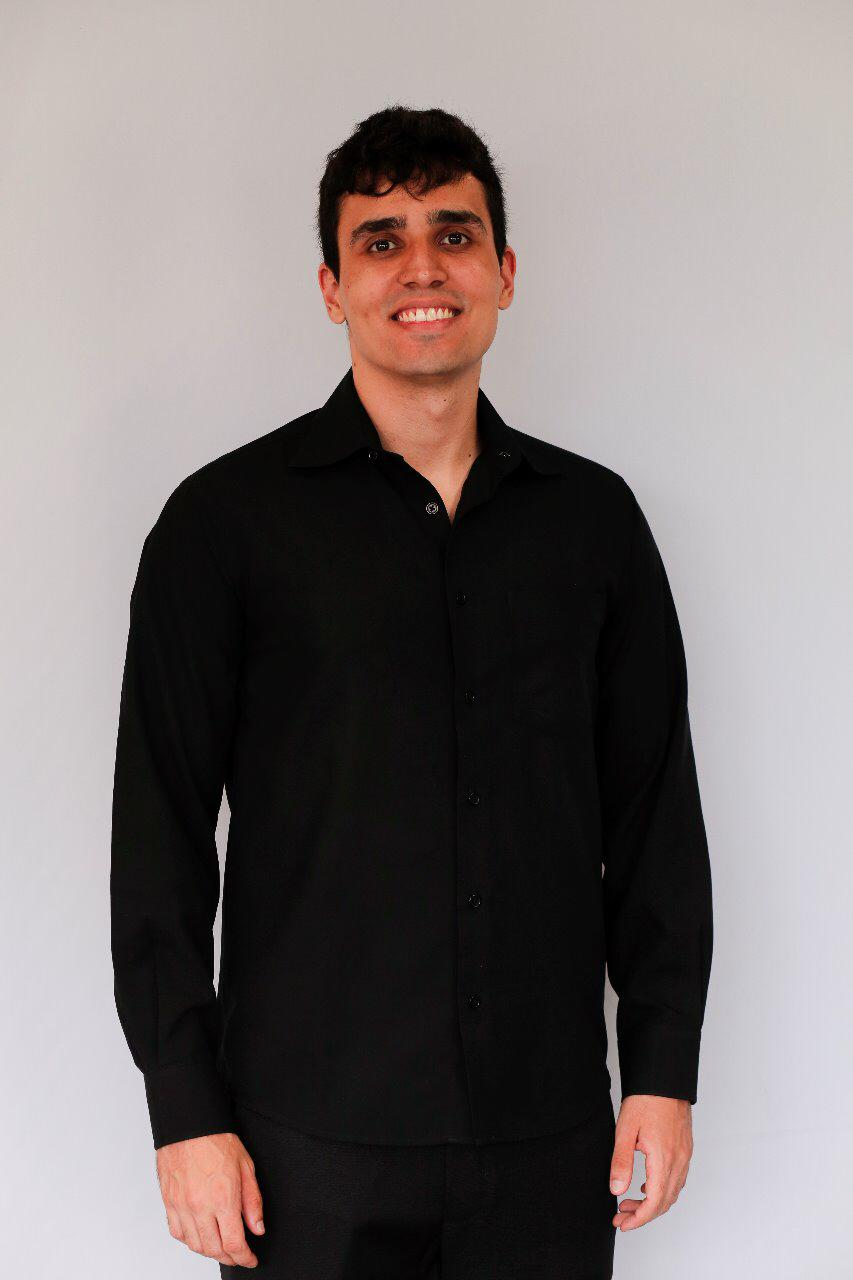
\includegraphics[width=\linewidth]{img/profile.jpeg}
	\end{minipage}
	\hspace*{-3.35\fboxrule}
	}
	\hfill
	\begin{minipage}{0.65\linewidth}
		\Huge{\bf \professional, \age}\\\vspace{-1.75\baselineskip}

		\noindent\rule{\textwidth}{1.5pt} {\ }\\\vspace{-1.8\baselineskip}

		\large{
		\faMapMarker \ \address \\
		\begin{minipage}{0.5\linewidth}
			\faWhatsapp \ \phone
		\end{minipage}
		\begin{minipage}{0.5\linewidth}
			\faEnvelope \ \email
		\end{minipage}
		\begin{minipage}{0.5\linewidth}
			\faLinkedinSquare \ \href{https://www.linkedin.com/in/mateusoliveira43/}{\texttt{/mateusoliveira43}}
		\end{minipage}
		\begin{minipage}{0.5\linewidth}
			\faGithub \ \href{https://github.com/mateusoliveira43}{\texttt{/mateusoliveira43}}
		\end{minipage}
		\faLink \ \href{https://mateusoliveira43.github.io/}{\texttt{mateusoliveira43.github.io}}\\
		\vfill
		\textbf{About}:\about
		}
	\end{minipage}
	\vspace{\baselineskip}

%%%%%%%%%%%%%%%%%%%%%% - CV's Body - %%%%%%%%%%%%%%%%%%%%%%
    \createSection[1]{Education}{2}{
		\textit{Mathematics - Bachelor Degree}, Federal University of Santa Catarina (UFSC), Florianópolis, Santa Catarina \hfill 2014 - 2020 \\
	}

	\createSection[1]{Experience}{21}{
	    \textit{Junior Software Developer}, Fundação CERTI, Florianópolis, Santa Catarina \hfill October 2020 - currently \\
	    \textbf{Activities}: Acting in a WEB project involving Python (FastAPI, SQLAlchemy) in the Backend, JavaScript (Node.js, React, TypeScript) in the Frontend, PostgreSQL in the database. All the code being continuous integrated by Jenkins, having quality measures by tests, linter and SonarQube and containerized with Docker. Planning and working following some of the agile methodologies principles. \\

	    \textit{Scientific Initiation Scholarship}, Federal University of Santa Catarina (UFSC), Florianópolis, Santa Catarina \hfill August 2019 - February 2020 \\
		\textbf{Activities}: Research focused in Computer Graphics.\\

		\textit{Laboratory of Mathematical and Technological Studies (LEMAT) Scholarship}, Federal University of Santa Catarina (UFSC), Florianópolis, Santa Catarina \hfill March 2019 - July 2019 \\
		\textbf{Activities}: Application, development and update of project files.\\

		\textit{Regional Mathematical Olympiad of Santa Catarina (ORM) Journal Scholarship}, Federal University of Santa Catarina (UFSC), Florianópolis, Santa Catarina \hfill March 2016 - March 2017 \\
		\textbf{Activities}: Application and development of training files; correction and development of test files; update of journal master file.\\

		\textit{Tutorial Education Program in Mathematics (PET Matemática) Scholarship}, Federal University of Santa Catarina (UFSC), Florianópolis, Santa Catarina \hfill March 2015 - February 2016 \\
		\textbf{Activities}: Application and development of training files; teaching in pre-university preparatory course; teaching and elaboration of \LaTeX\ and Matlab mini courses.\\
	}

    \createSection[1]{Programming languages and tools}{2}{
        \large{\bf
			\begin{minipage}{0.6\linewidth}
				Python (FastAPI and Django)\\
				JavaScript (Node.js, React and TypeScript)\\
				Git\\
				Linux\\
			\end{minipage}
			\begin{minipage}{0.4\linewidth}
				HTML\\
				CSS (Bootstrap)\\
				Docker\\
				PostgreSQL\\
			\end{minipage}
		}
    }

	\createSection{Languages}{2}{
	    \large{
			\begin{minipage}{0.5\linewidth}
				\textbf{Portuguese}: native \\
				\textbf{English}: fluent \\
			\end{minipage}
			\begin{minipage}{0.5\linewidth}
				\textbf{Spanish}: basic \\
				\textbf{German}: basic \\
			\end{minipage}
		}
	}
%%%%%%%%%%%%%%%%%%% - End of CV's Body - %%%%%%%%%%%%%%%%%%
    \label{lastPage}
\end{document}
